\section{METHODS}
\label{s:methods}
In the case of a tendon-driven limb with $n$ muscles, the feasible activation space is the unit $n$-hypercube (as muscles can only be activated positively from 0 to a maximal normalized value of 1). As explained in \cite{Valero-Cuevas2009mathematical}, when task constraints are introduced to the system, the feasible activation set is further reduced; in this context, a task is a static force vector produced at the endpoint of the limb, which is represented as a set of inequality and equality constraints. Thus if this simple limb meets all constraints, the feasible activation set is given by the polytope containing all $a \in \mathbb{R}^n$, that satisfy
\[\textbf{f} = A\textbf{a}, \textbf{a} \in [0,1]^n,\]
where $\textbf{f} \in \mathbb{R}^m$ is a fixed force vector and $A = J^{-T}RF_o \in \mathbb{R}^{m \times n}$--- where $J$, $R$ and $F_0$ are the matrices of the Jacobian of the limb, the moment arms of the tendons, and the strengths of the muscles, respectively \cite{Valero-Cuevas1998Large,Valero-Cuevas2009mathematical}. $P$ is bounded by the unit $n$-cube since all variables $a_i$, $i \in [n]$ are in the interval $[0,1]$.
Consider the following $1 \times 3$ fabricated example, where the task is a 1N unidimensional force.
\begin{align*}
&1 = \frac{10}{3}a_1 - \frac{53}{15}a_2 + 2a_3 \\
&a_1, a_2, a_3 \in [0,1],
\end{align*}

\begin{figure}[schematic_arm]
  \label{fig:schematic_arm}
  \centering
  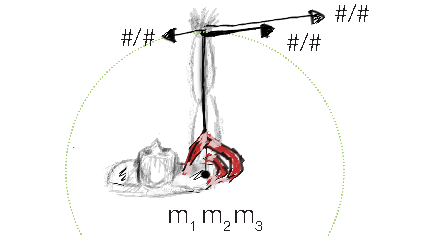
\includegraphics[width=0.5\textwidth]{sections/figs/schematic_example_drawing.pdf}
  \caption{One imagined visualization of the fabricated tendon driven system, with 3 generators.}
  \label{fig:finger}
\end{figure}


The set of feasible activations is given by the shaded set in Figure \ref{fig:fig_hr}.

\begin{figure}[ht]
  \label{fig:fig_hr}
   \begin{center}
    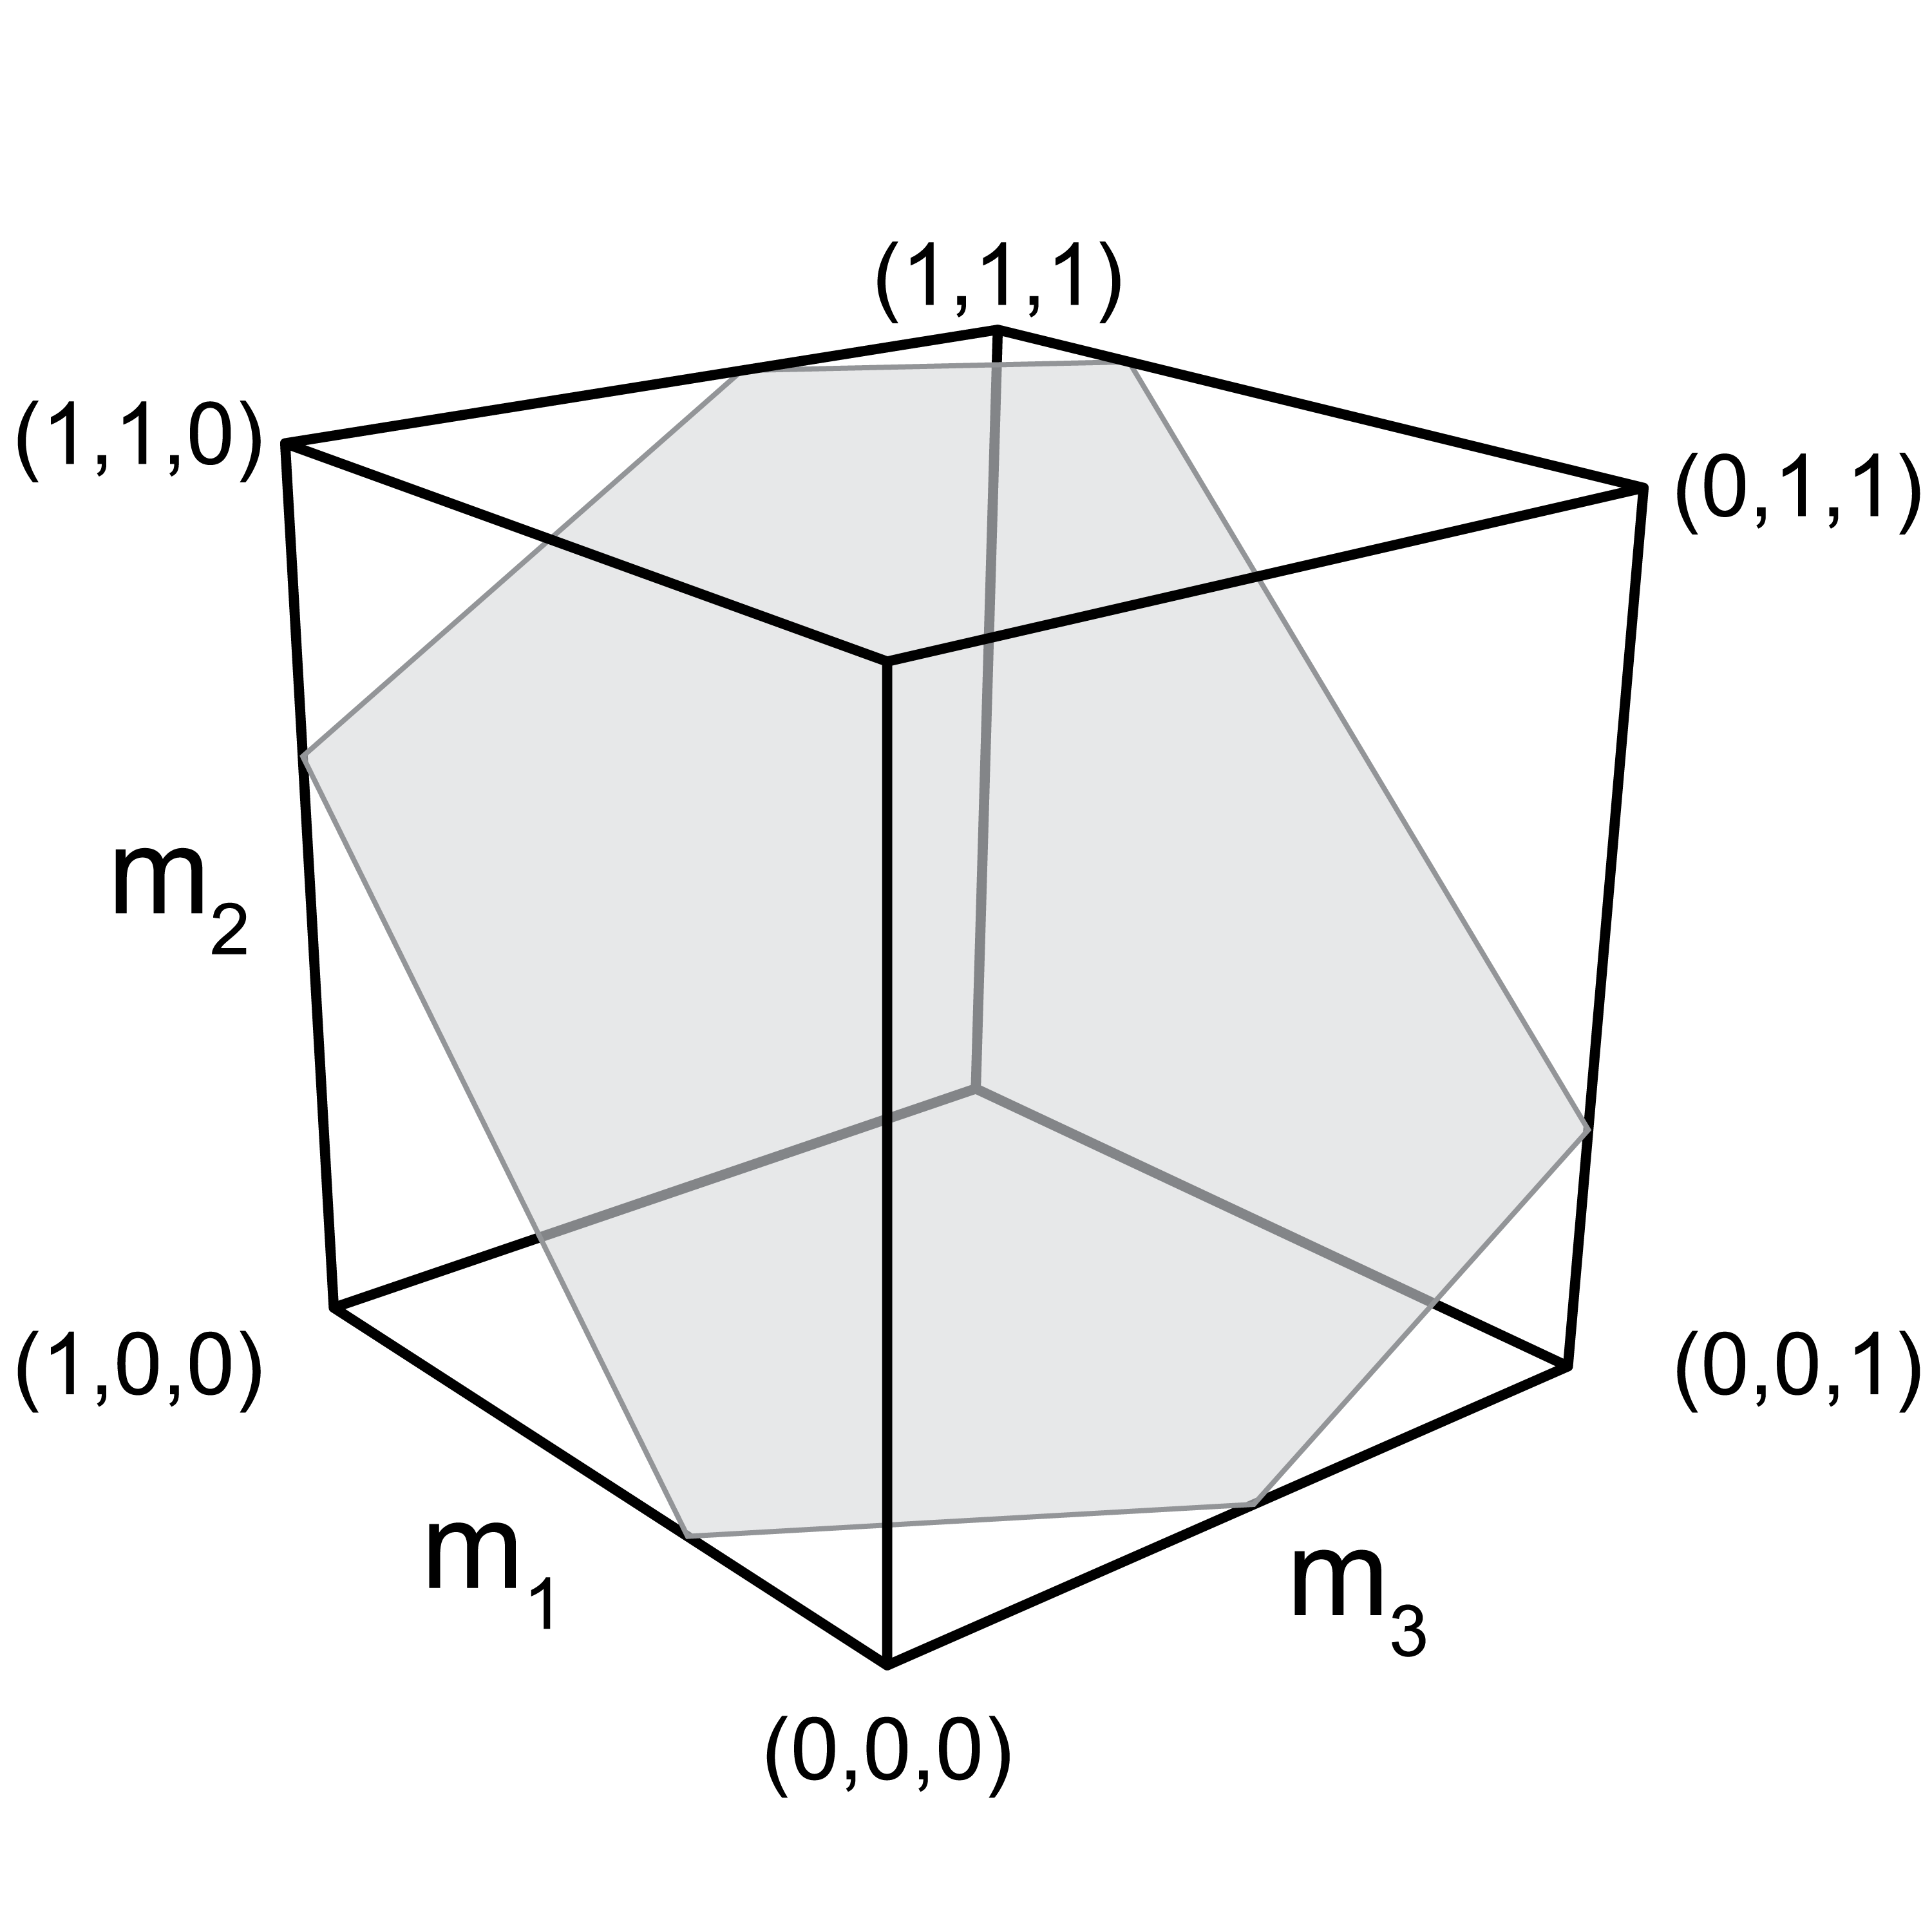
\includegraphics[width=0.25\textwidth]{sections/figs/feasibleactivation.png}
  \end{center}
  \caption{The feasible activation set for a  three-muscle system meeting one functional constraint is a polygon in $\mathbb{R}^3$.} %Note that muscle activations are assumed to be bounded between $0$ and $1$.}
\end{figure}

\subsection{Difficulty in multidimensional integration}

Exact volume computations for polytopes is know to be $P$-hard \cite{Dyer}. Several algorithms have been suveyed and implemented, but can only handle up to 10 dimensions \cite{Bueler2}.  
%We aimed to compare the relative volumes of different sections of the activation space; however, exact volume computations are computationally intractable in dimensions beyond [maytodo cite]. 
Recent models we have used have been 31 dimensions \cite{Valero-Cuevas2015high-dimensional}, and other muscle models have over 40 muscles involved \cite{arnold2010model, kutch2012challenges, hamner2010muscle, de2014human}, thereby limiting the feasibility of using direct volume computations. Instead, we chose to sample the continuous space, effectively approximating the volume of the polytope by calculating point densities. [maytodo mention whether the volume computation is a closed-form solution]

\subsection{Hit-and-Run algorithm}
We chose to sample the activation space with the Hit-and-Run method because it is known to converge to the uniform distribution across a convex body \cite{smith1984efficient}. The Hit-and-Run method is a generalization of the discrete Markov chains. The mixing time is known to be $\mathcal{O}^*(n^2R^2/r^2)$, where $R$ and $r$ are the radii of the inscribed and cicumscribed ball of $K$ respectively \cite{Dyer, Lovasz}. I.e., after $\mathcal{O}^*(n^2R^2/r^2)$ steps, the Hit-and-Run algorithm has sampled a point uniformly at random (u.a.r.) in the convex body. Unfortunately the hidden constant is large, which makes the problem practically almost infeasible. However experimental results suggest that a number of points linear w.r.t.\ to the dimension suffices; this will be discussed in Section \ref{sec_lengthrun}.
As the feasible activation space of the muscles are given by a convex polytope, this method can be directly applied for our problem. Notably, there are other methods which sample uniformly; we chose Hit-and-Run because of [maytodo insert some other sampling paradigmns and our justification for Hit and run (include the Metropolis Hastings algorithm, Gibbs sampling?)].

[maytodo mention whether hit and run is a closed form solution]
%Hit-and-Run is a method used to uniformly sample a convex body \cite{smith1984efficient}. As the set of all feasible activations is defined by the mechanics of the limb and the constraints of the task (described in \ref{ss:finger}), we decided to use Hit-and-run to sample muscle activation solutions from the polytope $P$. We refer to each sample from $P$ as a 'point' $p \in [0,1]^n$.

The Hit-and-Run walk on $P$ is defined as follows (it works analogously for any convex body):
\begin{enumerate}
\item Find a starting point $\textbf{p}$ of $P$ %(Figure \ref{fig:hitruncube}a) .
\item Generate a random direction from $\textbf{p}$ in $P$ (uniformly at random over all directions) (Figure \ref{fig:hitruncube}a).
\item Find the intersection points of the random direction with the edges of the polytope (Figure \ref{fig:hitruncube}b).
\item Choose a point u.a.r.\ on this line segment given by the intersection points (Figure \ref{fig:hitruncube}c). 
\item Repeat from $1.$ the above steps with the new point as the starting point .
\end{enumerate}

\begin{figure}[htbp]
\centering
\includegraphics[width=0.5\textwidth,page=10]{sections/figs/HitandRunSchematics_all.pdf}
\caption{Graphical description of the Hit-and-Run algorithm.}
\label{fig:hitruncube}
\end{figure}

%\begin{figure}[htbp]
%\centering
%\includegraphics[width=0.5\textwidth,page=7]{sections/figs/HitandRunSchematics_all.pdf}
%\caption{Distribution of feasible activations for [briantodo: select task percent]50\% maximal force output in the palmar direction.}
%\label{fig:prebasis_cube}
%\end{figure}

%\begin{figure}[htbp]
%\centering
%\includegraphics[width=0.5\textwidth,page=8]{sections/figs/HitandRunSchematics_all.pdf}
%\caption{This shows how the basis vectors are orthogonal following Gram-Schmidt orthogonalization.}
%\label{fig:postbasis_cube}
%\end{figure}

\begin{figure}[htbp]
\centering
\includegraphics[width=0.5\textwidth,page=9]{sections/figs/HitandRunSchematics_all.pdf}
\caption{Uniform distribution aross the feasible activation space. In the schematic arm example, the distribution is represented within a 2D plane.}
\label{fig:posthitrun_distribution}
\end{figure}



\subsection{Implementation of Hit-and-Run}
To find a starting point in $P$ the polytope given by
\[\textbf{f} = A\textbf{a}, \textbf{a} \in [0,1]^n,\]
we only need to find a feasible activation vector. For the Hit-and-Run algorithm to mix faster we want the starting point not close to a corner. %centrally located point within the polytope- that way, the early points will not be clustered in a corner [maytodo cite]. 
We use the following standard trick with slack variables $\epsilon_i$, which for applications often gives a good starting point.% to select a point where activations $a_i$ for all muscles are far from 0 and 1, thereby finding a solution central within $P$ [maytodo cite the use of slack variables to improve mixing time].

\begin{equation}\label{eq:LP_r}
\begin{array}{lrcl}
\mbox{maximize} & \sum_{i=1}^n \epsilon_i \\ 
\mbox{subject to} & \textbf{f} &=& A\textbf{a}\\
  & a_i &\in& [\epsilon_i, 1- \epsilon_i], \hspace{5mm} \forall i \in \{1,\dots,n\}  \\
  & \epsilon_i &\geq& 0, \hspace{5mm} \forall i \in \{1,\dots,n\}.  
\end{array}
\end{equation}


The rest of the implementation of the Hit-and-Run algorithm is straight forward except for the choice of the random direction. How do we sample u.a.r.\ from all directions in $P$? Suppose that $\textbf{q}$ is a direction in $P$ and $p \in P$. Then by definition of $P$, $\textbf{q}$ must satisfy $\textbf{f} = A(\textbf{p}+\textbf{q})$. Since $\textbf{p} \in P$, we know that $\textbf{f} = A\textbf{p}$ and therefore 
\[\textbf{f} = A(\textbf{p} + \textbf{q}) = \textbf{f} + A\textbf{q}\]
and hence
\[A\textbf{q} = 0.\]

We therefore need to choose directions uniformly at random from all directions in the vectorspace 
\[V = \{\textbf{q} \in \mathbb{R}^n | A\textbf{q} = 0\}.\]

As shown by Marsaglia this can be done as follows \cite{Marsaglia}.

\begin{enumerate}
\item
Find an orthonormal basis $b_1, \dots, b_r \in \mathbb{R}^{n}$ of $A\textbf{q} =0$.
\item
Choose $(\lambda_1, \dots, \lambda_r) \in \mathcal{N}(0,1)^n$ (from the Gaussian distribution).
\item
$\sum_{i=1}^r \lambda_i b_i$ is a u.a.r.\ direction.
\end{enumerate}

A basis of a vectorspace $V$ is a minimal set of vectors that generate $V$, and it is orthonormal if the vectors are pairwise orthogonal (perpendicular) and have unit length. Using basic linear algebra one can find a basis for $V = \{A\textbf{q} = 0\}$ and orthogonalize it with the well known Gram-Schmidt method (for details see e.g.\ \cite{Robertson}). Note that in order to get the desired u.a.r.\ sample the basis needs to be orthonormal. For the limb case we can safely assume that the rows of $A$ are linearly independent and hence the number of basis vectors is $n-m$.
%\subsection{Removing inter-point dependence}
%\label{sec_lengthrun}
%As the function is recursive, any two successive points are not independent; therefore, we sample from our walk on $P$ by selecting every $m^{th}$ point to extract points which are distributed %uniformly-at-random across $P$, and are independent to eachother.
%Some have said that it takes X Hit-and-Run steps before the first and last points gathered are independent of one another, so we chose to collect every [maytodo confirm 100th] point into an array of points %$M = [p_0, p_1, p_2, ... p_{100,000}]$. 



\subsection{Mixing Time}
\label{sec_lengthrun}
A%lthough an increasing sample size of consecutive points will converge upon the uniform distribution of the polytope, we want to ensure that consecutive points are independent. [discussthis]How many points do we need to record from Hit-and-Run to reach a representative distribution across the polytope? 
From a given starting point, how many steps of the Hit-and-Run method are necessary to reach a u.a.r.\ point? For convex polygons in higher dimensions up to $40$, experimental results suggest that $\mathcal{O}(n)$ steps of the Hit-and-Run algorithm are sufficient.
In particular Emiris and Fisikopoulos paper suggest that $(10 + \frac{10}{n})n$ steps are enough to converge upon the uniform distribution \cite{emiris2013efficient}, while in Ge et al.'s paper every point of the Hit-and-Run algorithm is used in the sample \cite{Ge}. 
%With the index finger model we collected a sample of [briantodo number] points.


\subsection{Realistic index finger model}
\label{ss:finger}
We used our published model in \cite{Valero-Cuevas1998Large} to find matrix $A \in \mathbb{R}^{4 \times 7}$, where $\textbf{a} \in \mathbb{R}^7$; the four degrees of freedom were ad-abduction, flexion-extension at the metacarpophalangeal joint, and flexion-extension at the proximal and distal interphalangeal joints.
The force directions we simulated are visible in Figure \ref{fig:finger}. In this model, for each input we collected 1.000.000 points and sampled every 100th point. Our code only solves one linear equation to find the starting point, each step only needs time linear in the dimension. Therefore it can be used for other tendon driven models in higher dimension. [briantodo: please rephrase this crappy sentence] 

\begin{figure}[htbp]
  \centering
  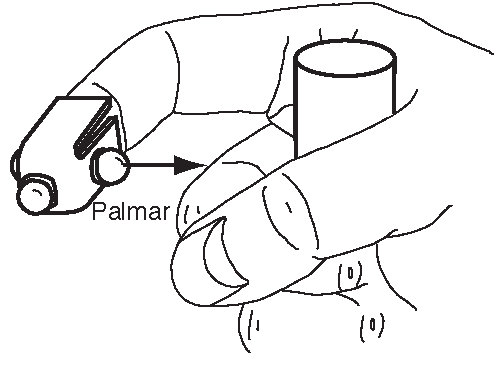
\includegraphics[width=0.5\textwidth]{sections/figs/finger.pdf}
  \caption{The index finger model simulated force production in the palmar direction. Adapted from \cite{Valero-Cuevas1998Large}.}
  \label{fig:finger}
\end{figure}



\subsection{Solution projection histograms}
The visualization for the distribution of solutions over each muscles is given in the histogramms in Figure\ref{fig:raw_histograms}. Since the generated points are uniformly at random distributed, this gives a close approximation. %The resulting array of points $M$ can be thought of as a matrix, where each row is a point, and each column is a muscle's activation. With this, we can enter a column of this data into a histogram; importantly, this approach projects the density of points. This can be used to approximate the relative volume of different sections of $P$- by slicing (binning) from each muscle's dimension.

\begin{figure}[htbp]
\centering
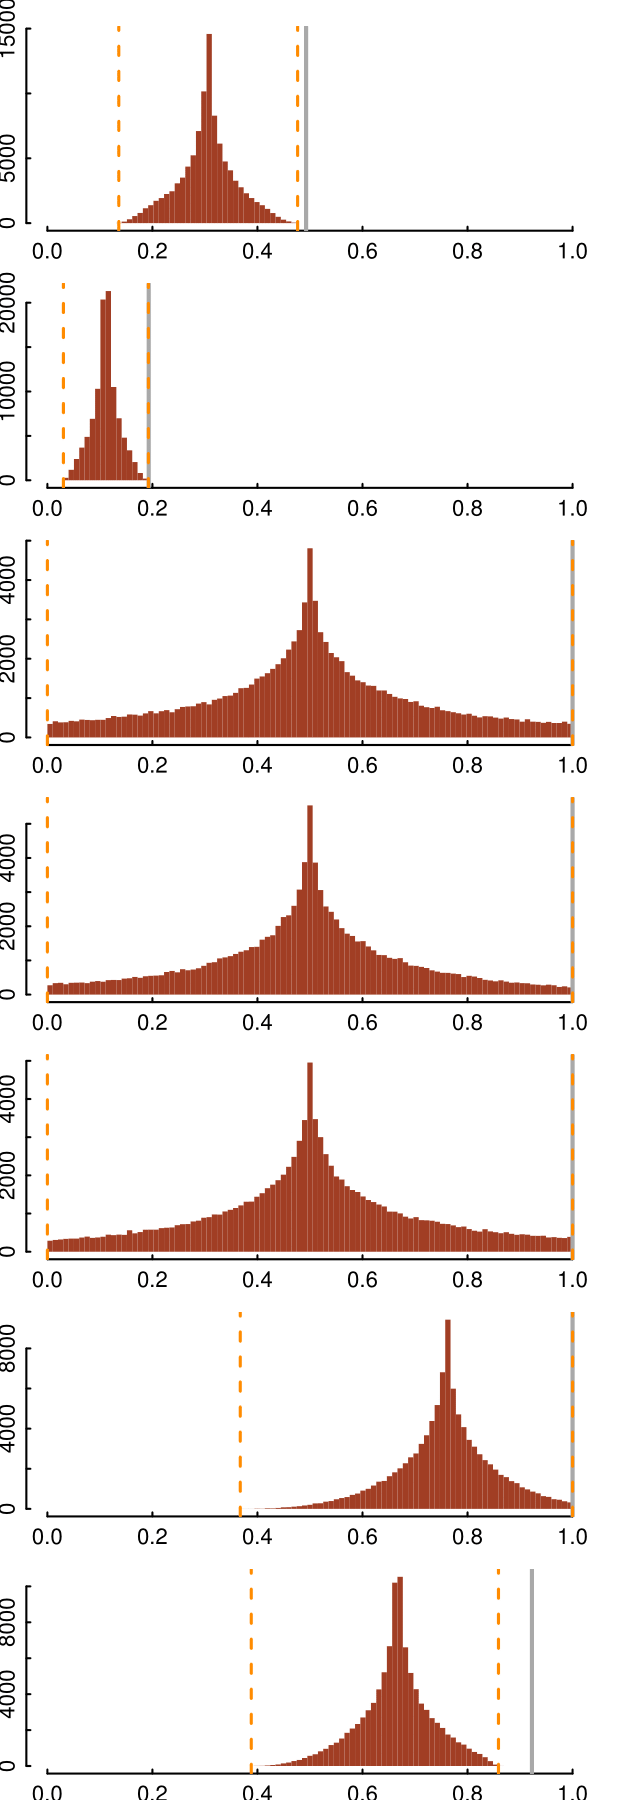
\includegraphics[width=0.5\textwidth]{sections/figs/raw_histograms.png}
\caption{Distribution of feasible activations for 50\% of the computed maximal force output in the palmar direction.}
\label{fig:raw_histograms}
\end{figure}

\subsection{Parallel coordinates visualization}
A common way to visualize higher dimensional data is using parallel coordinates[briantodo citations]. To show our sample set of points in the feasible activation space we draw $n$ parallel lines for each of the $n$ muscles. With the axis labels of the line set between 0 and 1, each point is then represented by connecting their coordinates by $n-1$ lines. Using an interactive surface we restrict each muscle function to any desired interval- see, figures [maytodo link these to result figures].

We decided to simulate a 50\% reduction in activation (feasible tendon force production) in three of the muscles innervated by the deep branch of the ulnar nerve- PI, DI, and FDP. 

\subsection{Muscle-metabolic and neural drive cost functions}

For every solution collected, we used popularly-used cost functions: we computed activation $l_1$, $l_2$ and $l_3$ norms, and the tendon-force $l_1^w$, $l_2^w$ and $l_3^w$ norms.


\begin{table}[h]
\centering
\begin{tabular}{@{}ll@{}}
\toprule
\textbf{Name} & \textbf{Cost function}  \\ \midrule
$l_1$            & $\sum_{i=1}^n a_i$                                     \\
$l_2$            & $\sqrt{\sum_{i=1}^n a_i^2}$                                    \\
$l_3$            & $\sqrt[3]{\sum_{i=1}^n a_i^3}$                                   \\
$l_1^w$            & $\sum_{i=1}^n a_i F_{0i}$                                    \\
$l_2^w$            & $\sqrt{\sum_{i=1}^n (a_i F_{0i})^2}$                                  \\
$l_3^w$            & $\sqrt[3]{\sum_{i=1}^n (a_i F_{0i})^3}$                                    \\ \bottomrule
\end{tabular}

\caption{Cost functions and their usage, where $a_i$ and $F_{0i}$ represent a muscle's activation in a given solution and that muscles MIC, respectively.}
\label{cost_function_tabls}

\end{table}

 Six additional vertical lines were added to the parallel coordinates plot to represent each cost function. With the same parallel coordinates framework as developed with muscle activation, we can restrict and subset solutions which fall into desired cost-function ranges, thereby masking sub-optimal solutions and highlighting only those meeting the criteria.

For a given point $\textbf{a} \in \mathbb{R}^n$ we are interested in the associated cost of every solution collected through Hit and Run.

We developed and tested our code in  Ubuntu 14.04, Windows 8.1, and OSX Yosemite, using Scala 2.11.6 [briantodo cite] for our implementation of Hit-and-Run, R 3.1.3 [briantodo cite] for histograms and plots, and using Sygmatic Parcoord[briantodo cite] and d3.js[briantodo cite] for our interactive parallel coordinate visualization. All code required to replicate our research is readily available at https://github.com/bcohn12/space.